\chapter{分次}\label{ch:grading}

上一章中，我们利用带标记曲面上的弧系定义了 $\mathbb Z_2$ 分次的 Fukaya 范畴。本章依照 Haiden、Katzarkov 和 Kontsevich\bookcite{115} 的工作，研究如何把这一构造提升到 $\mathbb Z$ 分次情形。这也使我们能够建立与真正簇而非 Landau--Ginzburg 模型之间的镜像对应；Lekili 和 Polishchuk 在文献\bookcite{165}中证明了这一点。

\section{分次曲面}\label{sec:graded-surfaces}
\takeaway{线场是射影切丛 $P T\dot S$ 的截面，曲线的分次就是相位 $\theta$ 的提升，平移 $[n]$ 把相位加 $n\pi$；只有绕数为 $0$ 的闭曲线可分次。标记点的指标由 $I_m=1-w/2$ 给出，并受 Poincaré 指标定理整体约束。}
\begin{definition}{分次带标记曲面}{graded-marked-surface}
分次带标记曲面\index{fencidaibiaojiqumian@分次带标记曲面|hyperpage} $\vec S$ 是一个三元组 $(S,M,\eta)$，其中 $(S,M)$ 是带标记曲面，而 $\eta$ 是一个光滑映射，它给每个点
\[
  p\in\dot S:=S\setminus M
\]
赋予切空间 $T_p\dot S$ 中的一个实一维子空间 $\eta_p$。映射 $\eta$ 称为\emph{线场\index{xianchang@线场|hyperpage}}或\emph{一维叶状结构}；它可以视为丛 $P T\dot S$ 的一个截面，其在 $p$ 上的纤维是射影直线 $\mathbb P(T_pS)$。满足对每个 $p\in L$ 都有 $T_pL=\eta_p$ 的一维子流形 $L\subset\dot S$，称为 $\eta$ 的叶。
\end{definition}

线场可用于定义分次弧\index{fencihu@分次弧|hyperpage}和分次曲线\index{kefenciquxian@可分次曲线|hyperpage}。为此，我们暂时在 $\dot S$ 上固定一个度量。该度量可以测量曲面上切向量之间的角度，并定义覆盖映射
\[
  \dot S\times\mathbb R\longrightarrow P T\dot S,\qquad (p,\theta)\longmapsto V_p,
\]
其中 $V_p\in P(T_p\dot S)$ 是与 $\eta_p$ 成角 $\theta$ 的一维子空间。在每个点 $p\in\dot S$ 上，此映射都是 $P(T_p\dot S)$ 的万有覆盖；当 $\theta_1-\theta_2$ 是 $\pi$ 的整数倍时，$(p,\theta_1)$ 与 $(p,\theta_2)$ 映到同一点。曲线的分次就是沿此覆盖映射对曲线作的一个提升。具体定义如下。

\begin{definition}{曲线的分次}{grading-of-curve}
设 $L\colon I\to S$ 是一条弧（此时 $I=(0,1)$）或一条闭曲线（此时 $I=\mathbb R/\mathbb Z$）。$L$ 的一个分次是映射 $\theta\colon I\to\mathbb R$，使得 $\theta(t)\bmod\pi$ 等于点 $p=L(t)$ 处线场 $\eta_p$ 与 $L$ 的切线之间的夹角。这个角称为相位。二元组 $\vec L=(L,\theta)$ 称为分次弧或分次曲线。其 $n$ 次平移定义为
\[
  \vec L[n]=(L,\theta+n\pi).
\]
% [Tutor Note: 平移下标按 $n\pi$ 而不是 $2\pi$：线场是无向的，相位只在模 $\pi$ 意义下有定义，所以 $\vec L[1]$ 是相位加 $\pi$（半圈）而非绕一整圈；$\mathbb Z$ 分次比 $\mathbb Z_2$ 分次多出的正是这一圈内的位置信息。]
\end{definition}

\begin{note}[度量的选择]
虽然上述定义看起来依赖度量，但不同度量所给出的覆盖映射 $\dot S\times\mathbb R\to P T\dot S$ 彼此同伦，因而可以在不同度量之间自然传递分次。
\end{note}

\begin{note}[沿曲线传递相位]
设 $L\colon I\to S$ 是一条曲线。若固定某个 $t\in I$ 处的 $\theta(t)$，则沿曲线传递夹角后，所有 $u\in(0,1)$ 处的相位都唯一确定：
\[
  \theta(u)=\theta(t)+\int_t^u
  \frac{d\angle(\dot L(s),\eta_{L(s)})}{ds}\,ds.
\]
记这一增量为 $\Delta_L[t,u]$。对弧 $L$，对任意
\[
  \theta(t)\in\angle(\dot L(t),\eta_{L(t)})+\pi\mathbb Z
\]
的选择都唯一确定一个分次，因此 $L$ 的分次与 $\mathbb Z$ 一一对应。

对闭曲线则更复杂。沿闭曲线 $L$ 传递相位后，相位一般会改变 $\pi$ 的整数倍。这个整数称为线场沿 $L$ 的绕数\index{raoshu@绕数|hyperpage}：
\[
  w(\eta,L)=\frac{\Delta_L[0,1]}{\pi}.
\]
要使分次良定义，绕数必须为 $0$；否则 $\theta\colon I\to\mathbb R$ 无法良定义。满足这一条件的闭曲线称为可分次闭曲线。与弧一样，可分次闭曲线的分次与 $\mathbb Z$ 一一对应。
\end{note}
% [Tutor Note: 绕数 $w(\eta,L)=\Delta_L[0,1]/\pi$ 必为整数：线场是 $P T\dot S$ 的截面，其纤维是长为 $\pi$ 的射影直线，沿闭曲线搬运一圈后相位只能相差 $\pi$ 的整数倍。$w\ne0$ 时不存在整体相位函数 $\theta$，这正是该曲线不可分次的原因。]

\begin{example}[向量场诱导的线场与指标]
若向量场 $V\colon S\to TS$ 的零点都在 $M$ 中，则令 $\eta_p=\mathbb R V_p$。向量场的积分曲线可取分次 $\theta=0$。对每个标记点 $m\in M$，取一条绕 $m$ 的小逆时针圆周 $\gamma_m$，并计算线场沿该圆周的绕数。$m$ 的指标定义为
\[
  I_m=1-\frac{w(\eta,\gamma_m)}{2}.
\]
当指标为 $1$ 时，这条小圆周可分次。更一般地，若 $S$ 中一条曲线围成圆盘 $D$，则它可分次当且仅当 $D$ 内所有标记点的指标之和为 $1$。

通常很容易确定标记点的指标。若标记点邻域内的向量场积分曲线绕着该点转动，则指标为 $1$。其余情形可将标记点邻域分成若干楔形区域，并按图\ref{fig:vector-field-index-wedges} 所示的三类楔形计数求和：
\begin{figure}[H]\centering
  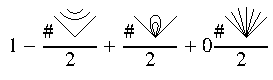
\includegraphics[width=0.42\textwidth]{figures/Fig_204_PDF308_Book296.pdf}
  \caption{由楔形区域计数确定标记点指标（原书 p.296）}\label{fig:vector-field-index-wedges}
\end{figure}

著名的 Poincaré 指标定理\index{poincarzhibiaodingli@Poincaré 指标定理|hyperpage}指出，这些指标之和等于 $S$ 的 Euler 示性数。
\end{example}

\begin{example}[复一形式定义的线场]
设 $S$ 是 Riemann 曲面，$\omega$ 是一个复一形式，并且它在 $M$ 之外没有零点或极点。令 $\eta_p\subset T_pS$ 为使 $\omega$ 取实值的一维子空间。在局部可取坐标 $z$ 使 $\omega=dz$，此时 $\eta_p$ 就是切空间中的实轴。

在零点或极点附近，$\omega$ 的形式为 $z^kdz$（$k\in\mathbb Z$）或 $\lambda z^{-1}dz$。相应线场的局部形状如图\ref{fig:one-form-line-fields} 所示；其指标为 $-k$。
\begin{figure}[H]\centering
  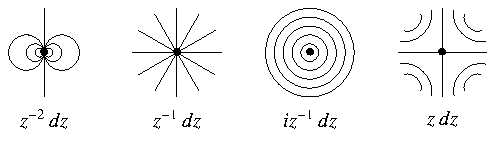
\includegraphics[width=0.72\textwidth]{figures/Fig_205_PDF309_Book297.pdf}
  \caption{$\omega$ 在零点和极点附近诱导的线场（原书 p.297）}\label{fig:one-form-line-fields}
\end{figure}
\end{example}

\begin{example}[二次微分定义的线场]\label{ex:quadratic-differential-line-fields}
也可以使用在 $M$ 外没有零点或极点的二次微分\index{erciweifen@二次微分|hyperpage} $\phi$。它是丛 $(T_{\mathbb C}^*S)^{\otimes2}$ 的一个截面。局部可写成
\[
  \phi=f(z)\,dz^2.
\]
若 $f(0)\ne0$，可换坐标使 $\phi=du^2$，并以新坐标中的切空间实轴定义 $\eta_p$。等价地，也可令 $\eta_p$ 是 $\phi$ 取正实值的方向；当 $\phi=f(z)dz^2$ 时，该方向为 $\mathbb R e^{-i\theta/2}$，其中 $\theta=\arg f(z)$。

在零点和极点附近，线场如图\ref{fig:quadratic-differential-line-fields} 所示。$z^kdz^2$ 的指标为 $-k/2$。注意，与向量场和一形式的情形不同，这些线场的指标可以是半整数。
\begin{figure}[H]\centering
  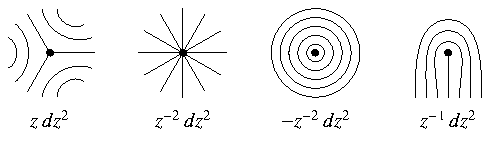
\includegraphics[width=0.72\textwidth]{figures/Fig_206_PDF309_Book297.pdf}
  \caption{二次微分在零点和极点附近诱导的线场（原书 p.297）}\label{fig:quadratic-differential-line-fields}
\end{figure}
\end{example}

\begin{definition}{线场的奇偶性}{line-field-parity}
若线场沿所有曲线的绕数都是偶数，或者等价地，该线场来自一个向量场，则称线场的奇偶性为偶；若至少有一条曲线的绕数为奇数，则称其奇偶性为奇。记线场 $\eta$ 的奇偶性\index{xianchangdejiouxing@线场的奇偶性|hyperpage}为 $\sigma(\eta)\in\mathbb Z/2\mathbb Z$。
\end{definition}
% [Tutor Note: 来自向量场的线场其绕数必为偶数：向量场方向以 $2\pi$ 为周期，而线场只以 $\pi$ 为周期，故沿任何闭曲线向量场转过的 $2\pi$ 整数倍对应线场 $w$ 的偶数。配合 $I_m=1-w/2$，这保证向量场给出的指标都是整数；一般线场的指标可以是半整数。]

设 $A$ 是剖分分次曲面 $\vec S$ 的弧系。为每条弧选定一个分次，并把所得分次弧集合记为 $\vec A$。若标记点 $p$ 处的角 $\alpha$ 位于分次弧 $\vec a=(a,\theta_a)$ 与 $\vec b=(b,\theta_b)$ 之间，则定义
\[
  \deg_{\vec A}\alpha
  :=\frac{\Delta_\alpha-(\theta_b(p)-\theta_a(p))}{\pi},
\]
其中 $\Delta_\alpha$ 是沿对应于角 $\alpha$ 的小圆弧移动时线场的变化量。由此得到的分次使温和代数的 $A_\infty$ 结构相容。

\begin{note}[角态射的分次]
上述定义同样不依赖测量角度所用度量。还可以这样定义：若 $\alpha\colon L_1\to L_2$ 是角态射，就沿路径 $\alpha$ 对 $L_1$ 作同位变形，得到一条新曲线 $L_1'$，使其端点与 $L_2$ 的端点重合；同时沿同位变形传递 $L_1$ 的分次。态射 $\alpha$ 的次数是使 $L_1'$ 的分次与 $L_2[n]$ 在重合端相同的整数平移量 $n$。
\end{note}

\begin{lemma}{高阶乘积的次数}{graded-higher-product-degree}
乘积 $\mu^k$ 关于 $\deg_{\vec A}$ 的次数为 $2-k$。
\end{lemma}
\begin{proof}[证明思路]
对 $\mu^2$，次数的可加性是显然的。若 $\alpha_1,\ldots,\alpha_k$ 是一个多边形的内部角，则它们的乘积是某条弧的恒等态射，故次数为 $0$。为确定各个 $\alpha_i$ 的总次数，可选取使该多边形成为平面的度量。此时结论等价于 $k$ 边形内角和为 $(k-2)\pi$。
\hfill$\square$
\end{proof}
% [Tutor Note: 度量可自由选取是关键一步：在多边形内部取平坦度量后，线场相位绕各角的变化只由内角决定，因此 $\sum_i\deg\alpha_i=k-2$ 与外角和恒为 $2\pi$（即内角和 $(k-2)\pi$）是同一件事。]

\begin{example}[球面上的一组分次]\label{ex:sphere-arc-grading}
上一章中，弧系所对应的温和代数带有由弧定向诱导的 $\mathbb Z_2$ 分次，但该分次不一定与线场给出的分次相容。

例如，取 Riemann 球面 $S=\widehat{\mathbb C}$，二次微分
\[
  \phi=(1-z^2)^{-1}dz^2,
\]
与标记点集 $M=\{-1,1,\infty\}$。这三个标记点的指标分别为 $1/2,1/2,1$；对于最后一个点，令 $z=u^{-1}$，则
\[
  \phi=u^{-2}(u^2-1)^{-1}(du)^2,
\]
故其指标为 $-(-2/2)=1$。

弧系可取扩充实轴 $\widehat{\mathbb R}\subset\widehat{\mathbb C}=S$，它由三条弧
\[
  a_1=[\infty,-1],\qquad a_2=[-1,1],\qquad a_3=[1,\infty]
\]
组成。因为 $z^{-1}(1-z)^{-1}$ 在 $(0,1)$ 上为正，线场与 $a_2$ 平行，而与 $a_1,a_3$ 垂直。因此可取 $\theta_{a_1}=\theta_{a_3}=\pi/2$、$\theta_{a_2}=0$。绕 $-1$ 或 $1$ 转半圈时，线场改变 $\pi/2$，于是
\[
\begin{aligned}
  \deg_{\vec A}\alpha_{-1}^{+}&=1,&
  \deg_{\vec A}\alpha_{-1}^{-}&=0,\\
  \deg_{\vec A}\alpha_{1}^{+}&=0,&
  \deg_{\vec A}\alpha_{1}^{-}&=1.
\end{aligned}
\]
绕 $\infty$ 的角处线场没有变化，所以
\[
  \deg_{\vec A}\alpha_{\infty}^{+}
  =\deg_{\vec A}\alpha_{\infty}^{-}=0.
\]
这三条弧把球面剖分成两个三角形，每个三角形内部角的次数之和都是 $1+0+0=3-2$，符合要求。
\begin{figure}[H]\centering
  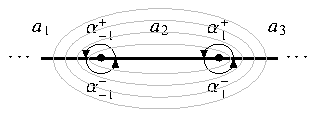
\includegraphics[width=0.34\textwidth]{figures/Fig_207_PDF311_Book299.pdf}
  \caption{球面弧系及其角的分次（原书 p.299）}\label{fig:sphere-arc-grading}
\end{figure}

这一分次与弧系的 $\mathbb Z_2$ 分次不相容：$\alpha_{-1}^{+}\alpha_{-1}^{-}$ 是从 $a_1$ 到自身、绕标记点转一整圈的态射，其 $\mathbb Z_2$ 次数为 $0$，而线场分次下两角次数之和为 $1$。
\end{example}

\begin{example}[为任意温和代数分次构造线场]\label{ex:line-fields-arbitrary-gradings}
若弧系中的弧同时是线场的叶\index{xianchangdeye@线场的叶|hyperpage}，则只需令 $\theta_a\equiv0$，便能很容易地给弧分次。角态射的次数也容易确定：在每个标记点附近把曲面分成楔形区域，角的次数就是它穿过的各类楔形区域的带符号计数，见图\ref{fig:grading-by-wedges}。
\begin{figure}[H]\centering
  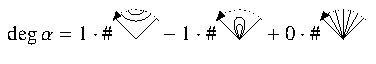
\includegraphics[width=0.42\textwidth]{figures/Fig_208_PDF311_Book299.pdf}
  \caption{由楔形区域计算角态射次数（原书 p.299）}\label{fig:grading-by-wedges}
\end{figure}

反过来，设 $A$ 是弧系，其温和代数 $\mathrm{Gtl}^{\bullet}A$ 上给定一个次数函数 $\deg\colon Q_1\to\mathbb Z$，并且每个 $k$ 边形中各角次数之和为 $k-2$。那么可以构造出与此分次对应的线场。首先，添加对角线可将问题化为所有多边形均为三角形的情形。对一个三角形，设
\[
  \deg\alpha_1+\deg\alpha_2+\deg\alpha_3=3-2=1.
\]
最简单的次数配置 $(1,0,0)$ 显然可由图\ref{fig:triangle-line-fields} 中的线场实现。
\begin{figure}[H]\centering
  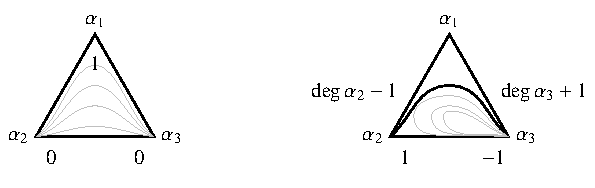
\includegraphics[width=0.78\textwidth]{figures/Fig_209_PDF311_Book299.pdf}
  \caption{三角形上的基本线场构造（原书 p.299）}\label{fig:triangle-line-fields}
\end{figure}
其余情形可对 $|\deg\alpha_1|+|\deg\alpha_2|+|\deg\alpha_3|$ 作归纳。选两个次数异号的角，例如 $\deg\alpha_2>0$、$\deg\alpha_3<0$。在这两个角之间画一条新弧，并在新的二边形内填入泪滴形线场；图\ref{fig:triangle-line-fields} 右侧展示了这一步。剩余三角形的角次数应为 $\deg\alpha_1,\deg\alpha_2-1,\deg\alpha_3+1$。
\end{example}

\begin{theorem}{剖分弧系所给出的导出等价}{graded-arc-collections-equivalent}
\textnormal{（\bookcite{115}）}
若 $\vec A$ 与 $\vec B$ 是分次曲面 $\vec S$ 上两组剖分曲面的分次弧系，则
\[
  D\mathrm{Gtl}^{\bullet}\vec A\simeq D\mathrm{Gtl}^{\bullet}\vec B
\]
作为 $A_\infty$ 范畴等价。
\end{theorem}
\begin{proof}[证明思路]
证明与定理\ref{thm:gentle-derived-invariance} 完全类似。首先，不同分次的弧对应于对象的平移。若两条弧同位，则可沿同位变形把一条弧的分次传递到另一条弧；带有传递后分次的第二条弧与第一条弧同构。最后，在多边形中，可把一条对角线识别为边界弧的锥；适当选择边界弧的分次，使这些弧之间的角态射次数全为 $1$，则添加、删除或翻转对角线都不改变导出范畴。任意两组极大弧系可由一系列翻转连接，结论遂得。
\hfill$\square$
\end{proof}

\section{弦与带}\label{sec:graded-strings-bands}
\takeaway{分次弦对象的平移须满足 $i_{j+1}=i_j+\deg\alpha_j-1$；闭曲线还要求 $\sum_j(\deg\alpha_j-1)=0$，此时带对象由分次闭曲线与绕行变换决定。$D\mathrm{Gtl}^{\bullet}A$ 中每个对象都同构于弦对象与带对象的直和。}
与 $\mathbb Z_2$ 分次情形一样，可以构造弦对象和带对象
\[
  \left(\bigoplus_{j=1}^{k}a_j[i_j]^{\oplus n_j},\quad
  \delta=\sum_{j=1}^{k}\lambda_j\alpha_j\right),
\]
但现在必须谨慎选取平移 $i_j$：所有 $\alpha_j$ 都必须是次数为 $1$ 的态射。若任意固定 $i_1$，则对每个 $j\ge1$ 令
\[
  i_{j+1}=i_j+\deg\alpha_j-1.
\]
弦对象总能如此分次，因此对于每个 $i_1\in\mathbb Z$，每个弦对象都恰有一种相应的分次。

给定弦对象，可以构造一条沿着各条 $a_j$ 延伸、并避开标记点小邻域的弧。在这些小邻域内，新弧先向右转 $90$ 度，再沿一段圆弧转过角 $\alpha$，然后再向右转 $90$ 度。沿这条变形后的路径传递相位时，若 $\alpha_j$ 的次数为 $1$，相邻 $a_j$ 之间的相位便会吻合，因为该次数恰好抵消两次右转的贡献。所得分次弧表示这个弦对象；当所有弧的相位均为 $0$ 时，这一构造最容易看清。其示意如图\ref{fig:graded-string-arc} 所示。
\begin{figure}[H]\centering
  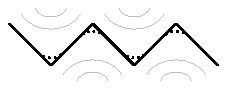
\includegraphics[width=0.32\textwidth]{figures/Fig_210_PDF312_Book300.pdf}
  \caption{分次弦对象对应的弧示意图（原书 p.300）}\label{fig:graded-string-arc}
\end{figure}

对于带对象，弧的指标是循环的，因此必须有 $i_{j+k}=i_j$。这只有在
\[
  \sum_j(\deg\alpha_j-1)=0
\]
时才可能。此时所得曲线可分次，上述过程会给出一条分次闭曲线。因此，带对象由分次曲线 $\vec L$ 与其局部系统的绕行变换 $T_\lambda$ 决定。反之，给定一条分次弧或带局部系统的闭曲线，可将其同位变形成一列弧与角，并沿同位变形传递分次，进而将该弧或闭曲线识别为弦对象或带对象。这个对应也反向成立。

\begin{theorem}{弦与带对象的分解定理}{graded-string-band-decomposition}
\textnormal{（Haiden--Katzarkov--Kontsevich）}设 $(\vec S,M)$ 是带标记点的分次曲面，$\vec A$ 是剖分该曲面的分次弧系。$D\mathrm{Gtl}^{\bullet}\vec A$ 中的每个对象都同构于弦对象与带对象的直和。
\end{theorem}
\begin{proof}[证明思路]
分两步证明。第一步只考虑没有内部标记点的曲面。此时可选择一组弧系，使其箭图没有有向环，因此不存在高阶 $\mu$ 乘积，且 $\mathrm{Gtl}^{\bullet}A$ 是有限维的。于是可以使用普通分次温和代数的标准方法（见\bookcite{192,197,115}）。

对于含内部标记点的情形，在该标记点周围切出一个小圆，并在新圆周上添加一个标记点。记所得曲面为 $(S',M')$，并将线场限制到其上。$(S',M')$ 上的每个分次弧系 $\vec A'$ 也可看作 $(S,M)$ 上的弧系 $\vec A$。如定理\ref{thm:tubular-graph-sheaf-functor} 的构造，可得一个 $A_\infty$ 函子
\[
  \phi\colon\mathrm{Gtl}^{\bullet}A'\longrightarrow\mathrm{Gtl}^{\bullet}A,
\]
它在导出范畴上诱导本质满函子（见\bookcite{115}）。因此，$D\mathrm{Gtl}^{\bullet}A$ 中每个对象都来自 $D\mathrm{Gtl}^{\bullet}A'$ 中弦对象与带对象的直和。在函子 $D\phi$ 下，$(S',M')$ 中的弦或带被切成若干段，这些段包含在 $(S,M)$ 中，并分别给出弦对象或带对象。
\hfill$\square$
\end{proof}

\begin{definition}{分次曲面的拓扑 Fukaya 范畴}{graded-topological-fukaya}
分次曲面的拓扑 Fukaya 范畴\index{tuopufukayafanchou@拓扑 Fukaya 范畴|hyperpage}定义为
\[
  \mathrm{topFuk}^{\bullet}(\vec S,M):=D\mathrm{Gtl}^{\bullet}\vec A,
\]
其中 $\vec A$ 是任意一组剖分曲面的分次弧系。
\end{definition}

\section{分次曲面的刻画}\label{sec:characterizing-graded-surfaces}
\takeaway{线场的同位类构成 $\mathrm{LF}(S,M)$，映射类群作用后得 $\mathrm{MLF}(S,M)$；不变量（奇偶性、绕数向量 $W$，$g=1$ 时的 $\mathrm{GCD}$ 与 $g\ge2$ 时的 $\mathrm{ARF}$）完全刻画线场，从而可判定两个分次曲面是否等价。}
\begin{definition}{分次曲面的等价}{graded-surface-equivalence}
若两个线场 $\eta_0,\eta_1$ 可由一条线场路径 $\gamma\colon[0,1]\to\Gamma(P T\dot S)$ 连接，即 $\gamma(t)=\eta_t$，则称它们同位。若两个分次曲面 $(S_1,M_1,\eta_1)$ 与 $(S_2,M_2,\eta_2)$ 之间存在微分同胚 $\phi\colon S_1\to S_2$，它将 $M_1$ 映到 $M_2$，且 $\eta_2$ 与 $\phi^*\eta_1$ 同位，则称这两个分次曲面等价。
\end{definition}

等价的分次曲面给出等价的 wrapped Fukaya 范畴。事实上，若 $A_1$ 是 $S_1$ 上的弧系，则 $A_2=\phi(A_1)$ 是 $S_2$ 上的弧系；利用 $\phi^*\eta_1$ 与 $\eta_2$ 之间的同位，可以传递分次。因此，$\mathrm{topFuk}^{\bullet}(\vec S_1,M_1)$ 和 $\mathrm{topFuk}^{\bullet}(\vec S_2,M_2)$ 都由同一个分次温和代数生成。

要判断两个分次曲面是否等价并不总是容易，因此需要一组能刻画其等价类的不变量。Lekili 和 Polishchuk 在文献\bookcite{166}中研究了这个问题。

\begin{definition}{线场的映射类不变量}{mapping-class-line-field-invariant}
对带标记曲面 $(S,M)$，记同位意义下线场的集合为
\[
  \mathrm{LF}(S,M):=\pi_0\bigl(\Gamma(P T\dot S)\bigr).
\]
映射类群
\[
  \mathrm{MCG}(S,M):=\pi_0\{\phi\in\mathrm{Diff}^+(S,S)\mid
    \forall m\in M,\ \phi(m)=m\}
\]
作用于该集合。记其轨道集为
\[
  \mathrm{MLF}(S,M):=\mathrm{LF}(S,M)/\mathrm{MCG}(S,M).
\]
取一组小逆时针圆周 $\Gamma$，其中每个内部标记点周围取一条、每个边界分支周围也取一条。映射类群固定标记点，因而也固定 $\Gamma$ 中这些曲线的同伦类。于是线场的绕数给出良定义映射
\[
  W\colon\mathrm{LF}(S,M)\longrightarrow\mathbb Z^{\Gamma},
\]
并且该映射经过轨道集 $\mathrm{MLF}(S,M)$。由 Poincaré 指标定理，$W$ 的像包含在子空间
\[
  \left\{a\in\mathbb Z^{\Gamma}\ \middle|\ \sum_{\gamma\in\Gamma}\left(1-\frac{a_\gamma}{2}\right)=2-2g\right\}
\]
之中。
\end{definition}

\begin{theorem}{分次带标记曲面的分类不变量}{graded-surfaces-classification}
\textnormal{（Lekili--Polishchuk\bookcite{166}）}设 $(S,M)$ 是亏格为 $g$ 的带标记曲面。两个线场 $\eta_1,\eta_2$ 对应于 $\mathrm{MLF}(S,M)$ 中同一点，当且仅当它们具有：
\begin{enumerate}[label=(\alph*)]
  \item 相同的奇偶性；
  \item 相同的绕数向量 $W(\eta_1)=W(\eta_2)$；
  \item 并满足下列附加条件：
  \begin{enumerate}[label=(\alph*\arabic*)]
    \item 若 $g=1$，则 $\mathrm{GCD}(\eta_1)=\mathrm{GCD}(\eta_2)$，其中
    \[
      \mathrm{GCD}(\eta)=\gcd\{w(\eta,\gamma)\mid
      \gamma\text{ 是闭曲线且 }S\setminus\operatorname{Im}\gamma\text{ 连通}\};
    \]
    \item 若 $g\ge2$ 且 $W(\eta_1)\in(2+4\mathbb Z)^{\Gamma}$，则
    \[
      \mathrm{ARF}(\eta_1)=\mathrm{ARF}(\eta_2),
    \]
    其中
    \[
      \mathrm{ARF}(\eta)=\sum_{i=1}^{g}
      \frac{w(\eta,\alpha_i)}{2}\frac{w(\eta,\beta_i)}{2}\pmod 2,
    \]
    而 $\alpha_i,\beta_i$ 是构成曲面辛基的一组闭曲线。
  \end{enumerate}
\end{enumerate}
\begin{figure}[H]\centering
  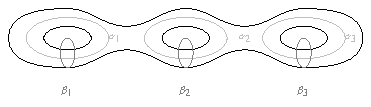
\includegraphics[width=0.48\textwidth]{figures/Fig_211_PDF315_Book303.pdf}
  \caption{曲面上的一组辛基曲线（原书 p.303）}\label{fig:symplectic-basis}
\end{figure}
\end{theorem}

\begin{note}[不变量与导出等价]
由于上述不变量刻画了弧系的分次曲面，它们可用于发现温和代数之间不明显的导出等价。具有相同不变量的温和代数导出等价；但反过来是否成立尚不清楚。温和代数之间或许还存在并非来自曲面等价的导出等价。更多细节及定理证明见文献\bookcite{166}。
\end{note}
\section{分次与矩阵分解}\label{sec:gradings-matrix-factorizations}
\takeaway{$B$ 侧把 $\mathbb Z$ 分次落在使势函数次数为 $2$ 的变量次数上（$\deg Z=2-\deg X-\deg Y$）；三标记球面的分次由 $\deg X=2-2I_{m_\xi}$ 等参数化，故分次裤子曲面镜像于带次数的 $(\mathbb C[X,Y,Z],XYZ)$，并可沿边界分支粘合、由格多边形与二聚体实现。}
在 $A$ 侧，$\mathbb Z$ 分次可以解释为线场；在 $B$ 侧，则需为矩阵分解范畴引入 $\mathbb Z$ 分次。带曲率代数中的零元乘积 $\mu^0$ 的次数为 $2$，因此要寻找使势函数次数为 $2$ 的分次。先从裤子曲面开始。

令 $(S,M)=(\mathbb P^1,\{0,\infty,1\})$。在 $\mathbb Z_2$ 分次情形，我们已知它与\linebreak Landau--Ginzburg 模型 $(\mathbb C[X,Y,Z],XYZ)$ 的矩阵分解范畴镜像。\linebreak 要得到 $\mathbb Z$ 分次版本，需给变量 $X,Y,Z$ 指定整数次数，使势函数的次数为 $2$。因此，固定 $\deg X,\deg Y$ 后必须令
\[
  \deg Z=2-\deg X-\deg Y.
\]
标准矩阵分解可以赋予相容分次：
\[
\begin{aligned}
  M_X&=\left(R\oplus R[1-\deg X],\begin{pmatrix}0&X\\YZ&0\end{pmatrix}\right),\\
  M_Y&=\left(R\oplus R[1-\deg Y],\begin{pmatrix}0&Y\\XZ&0\end{pmatrix}\right),\\
  M_Z&=\left(R\oplus R[1-\deg Z],\begin{pmatrix}0&Z\\XY&0\end{pmatrix}\right).
\end{aligned}
\]
态射
\[
  \zeta_1=\begin{pmatrix}0&-1\\Z&0\end{pmatrix}\colon M_X\longrightarrow M_Y
\]
的次数为 $1-\deg Y$，反向态射 $\zeta_2\colon M_Y\to M_X$ 的次数为 $1-\deg X$。它们的复合为
\[
  \zeta_1\zeta_2=
  \begin{pmatrix}-Z&0\\0&-Z\end{pmatrix}\colon M_Y\longrightarrow M_Y,
\]
其次数为 $2-\deg X-\deg Y=\deg Z$。在 $A$ 侧，这对应于绕标记点 $m_\zeta=1\in\{0,\infty,1\}$ 转过一个完整 $2\pi$ 角。按例\ref{ex:line-fields-arbitrary-gradings} 中的方法，可将两个三角形粘合起来，并令其内部角的次数分别为 $1-\deg X,1-\deg Y,1-\deg Z$。

另一方面，由定理\ref{thm:graded-surfaces-classification} 可知，三标记球面上的每种分次都由标记点周围的绕数确定。绕标记点的整周角次数为 $2-2I_m$，其中 $I_m$ 是该标记点的指标。因此，若令
\[
  \deg X=2-2I_{m_\xi},\qquad\ldots,\qquad
  \deg Z=2-2I_{m_\zeta},
\]
便可用分次 $B$ 模型实现每个分次 $A$ 模型。

\begin{theorem}{分次裤子曲面的镜像}{graded-pants-mirror}
分次带标记曲面
\[
  \bigl(\mathbb P^1,\{0,\infty,1\},z^k(z-1)^l dz^2\bigr)
\]
是如下分次 Landau--Ginzburg 模型的镜像：
\[
  (\mathbb C[X,Y,Z],XYZ),\qquad
  \deg X=2+k,\quad\deg Y=-k-l-2,\quad\deg Z=2+l.
\]
\end{theorem}

含有更多标记点且亏格更高的曲面，可由若干裤子曲面粘合而成；这个过程可以与分次相容。粘合两个裤子曲面的一条边界分支时，两侧整周角的次数必须互为相反数。满足这一条件后，可以同位变形线场\index{tongweibianxingxianchang@同位变形线场|hyperpage}使它们在交叠区域吻合：若裤子曲面某条边界分支的绕数为负数 $k$，可将其同位变形为 $k$ 个环绕楔形；坐标反演会把这些环绕楔形变成 $k$ 个鞍形楔形，对应正绕数，于是两侧在线场上吻合，得到连续线场。图\ref{fig:pants-line-field-gluing} 示意了这一过程。
\begin{figure}[H]\centering
  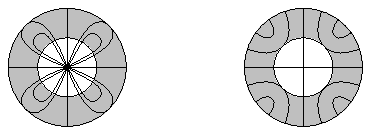
\includegraphics[width=0.55\textwidth]{figures/Fig_212_PDF316_Book304.pdf}
  \caption{粘合裤子曲面时的线场匹配（原书 p.304）}\label{fig:pants-line-field-gluing}
\end{figure}

这类曲面的镜像还可通过对格多边形作三角剖分来构造。如此得到带函数 $\ell$ 的三维环簇 $X$。多边形中的每个三角形 $\Delta$ 都给出一个矩阵分解
\[
  \bigl(\mathbb C[X_\Delta,Y_\Delta,Z_\Delta],X_\Delta Y_\Delta Z_\Delta\bigr),
\]
其中 $X_\Delta,Y_\Delta,Z_\Delta$ 是 $\mathbb C(U,V,W)$ 中的单项式，且
\[
  X_\Delta Y_\Delta Z_\Delta=W.
\]
若选取 $\deg U,\deg V\in\mathbb Z$ 并令 $\deg W=2$，便可定义 $(X,\ell)$ 的分次矩阵分解范畴；它与由分次裤子曲面粘合而成的分次曲面的 $A$ 模型等价。

\begin{example}[单位正方形的三角剖分]
考虑单位正方形，并将其分成两个三角形。这给出一个 Landau--Ginzburg 模型，其镜像是四穿孔球面，也就是两枚裤子曲面粘合而成的曲面。图\ref{fig:square-polygon-mirror} 标出了每个三角形外边对应的单项式；内边对应的单项式为 $UVW^{-1}$ 或其逆元。每条外边对应一个标记点，标记点的指标由相应单项式的次数确定；内边的次数则决定曲面上对应曲线的绕数。
\begin{figure}[H]\centering
  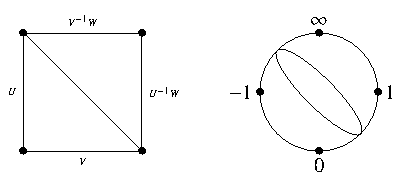
\includegraphics[width=0.68\textwidth]{figures/Fig_213_PDF317_Book305.pdf}
  \caption{正方形三角剖分及其四标记球面镜像（原书 p.305）}\label{fig:square-polygon-mirror}
\end{figure}
该例中的线场可由下列二次微分得到：
\[
  \phi=z^{\deg V-2}(z+1)^{\deg U-2}(z-1)^{-\deg U}\,dz^2.
\]
\end{example}

上一章还引入了非交换 Landau--Ginzburg 模型。若 $Q$ 是一致二聚体模型，可给 $Q$ 的每条箭赋予次数 $R_a$，并要求每个面上所有箭的次数之和为 $2$。于是，Jacobi 代数 $\mathrm{Jac}\,Q$ 可按此分次，$(\mathrm{Jac}\,Q,\ell)$ 成为分次非交换 Landau--Ginzburg 模型。每条箭对应的标准矩阵分解都可赋予分次，其箭映射如图\ref{fig:graded-dimer-matrix-factorization} 所示。
\begin{figure}[H]\centering
  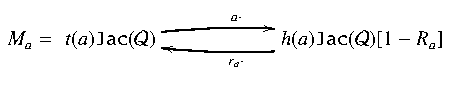
\includegraphics[width=0.63\textwidth]{figures/Fig_214_PDF317_Book305.pdf}
  \caption{二聚体箭所对应的分次矩阵分解（原书 p.305）}\label{fig:graded-dimer-matrix-factorization}
\end{figure}
相应地，态射 $\alpha\colon M_a\to M_b$ 由矩阵
\[
  \begin{pmatrix}0&-1_{t(a)}\\r_{ab}&0\end{pmatrix}
\]
表示，其次数为 $1-R_b$。对每个 $k$ 边形 $f\in Q_2$，该面内角态射的总次数为
\[
  \sum_{b\in f}(1-R_b)=k-2,
\]
因此可以构造一个边为线场叶、角次数与之相符的多边形。按二聚体对偶方式粘合这些多边形，就得到分次带标记曲面及其分次弧系，并且
\[
  \operatorname{End}^{\bullet}\left(\bigoplus_a M_a\right)
  \cong_\infty\mathrm{Gtl}^{\bullet}Q^\vee.
\]

\begin{example}[二聚体分次与对偶线场]
回到例\ref{ex:two-square-dimer} 中的二聚体 $Q$，令
\[
  \deg a_1=\deg a_2=\deg b_1=0,\qquad \deg b_2=2.
\]
在这一分次下，除终点为 $b_2$ 的角态射外，其余角态射次数都为 $1$。在对偶箭图中，可在这些特殊角处放置环绕楔形，在其他角处放置鞍形楔形。$Q^\vee$ 的四个顶点指标依次为 $1,0,0,1$；若将这些点分别识别为 $0,+1,-1,\infty\in\widehat{\mathbb C}$，所得线场与 $z^{-2}dz^2$ 同位。
\begin{figure}[H]\centering
  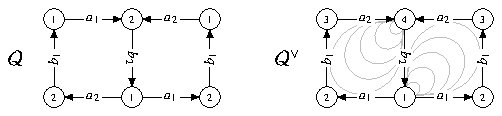
\includegraphics[width=0.71\textwidth]{figures/Fig_215_PDF317_Book305.pdf}
  \caption{二聚体及其对偶上的分次对应（原书 p.305）}\label{fig:graded-dimer-duality-example}
\end{figure}
\end{example}

\section{镜像簇}\label{sec:mirror-varieties}
\takeaway{当无边界曲面上各标记点的绕数只取 $0$（指标 $1$）或 $2$（指标 $0$）时，$\mathrm{topFuk}^{\bullet}$ 可等价于真正的（可能奇异的）簇的导出范畴：裤子曲面对应 $\mathbb A^1\cup_p\mathbb A^1$，直线链、射影直线环链与结点三次曲线都是这样得到的镜像。}
使用线场的一个优点是，在某些特殊情形下，我们可以超越矩阵分解的范畴，构造真正的簇作为镜像。在第\ref{ch:quivers}章的\hyperref[sec:points-sheaves]{“点与层”一节}中，我们看到，$\mathbb P^1$ 的导出范畴可解释为圆柱的拓扑 Fukaya 范畴；圆柱两侧各有一个标记点，线场平行于圆柱轴线。若把其中一个或两个边界分支收缩为内部标记点，所得范畴分别是 $\mathbb A^1$ 或 $\mathbb C^*=\mathbb A^1\setminus\{0\}$ 的导出范畴。

若允许奇异簇，这些例子可推广到没有边界分支、且标记点处绕数仅为 $0$（即指标为 $1$）或 $2$（即指标为 $0$）的分次带标记曲面 $(\vec S,M)$。由 Poincaré 指标定理，这只可能发生在以下两种情形：
\begin{itemize}
  \item $g=0$，此时恰有两个点的绕数为 $0$；
  \item $g=1$，此时没有点的绕数为 $0$。
\end{itemize}
此外，绕数为 $0$ 的点还可以改成各带一个标记点的边界分支。更多细节见\bookcite{232,165}；下面介绍几个例子。

再次从裤子曲面出发。可以把它看成 $(\mathbb P^1,\{0,1,\infty\})$，并取由一形式 $z^{-1}dz$ 给出的径向线场；此时 $0$ 与 $\infty$ 处的绕数为 $0$，而 $1$ 处的绕数为 $2$。我们断言：

\begin{lemma}{裤子曲面与相交直线的镜像}{graded-pants-two-lines-mirror}
分次曲面
\[
  (\mathbb P^1,\{0,1,\infty\},z^{-1}dz)
\]
的拓扑 Fukaya 范畴等价于两条仿射直线相交于一点的相干层导出范畴：
\[
  \mathrm{topFuk}^{\bullet}(\mathbb P^1,\{0,1,\infty\},z^{-1}dz)
  \cong_\infty D\mathrm{Coh}^{\bullet}(\mathbb A^1\cup_p\mathbb A^1)
  \cong_\infty D\mathrm{Mod}^{\bullet}\bigl(\mathbb C[X,Y]/(XY)\bigr).
\]
\end{lemma}
\begin{proof}[证明思路]
令 $R=\mathbb C[X,Y]/(XY)$，并考虑三个模
\[
  R,\qquad M_X=R/(X),\qquad M_Y=R/(Y).
\]
后两个模有如下周期分解，可用来计算 Ext 的 $A_\infty$ 代数：
\[
  \cdots\xrightarrow{X}R\xrightarrow{Y}R\xrightarrow{X}R\longrightarrow M_X,
  \qquad
  \cdots\xrightarrow{Y}R\xrightarrow{X}R\xrightarrow{Y}R\longrightarrow M_Y.
\]
该 Ext 代数由六个态射生成，其中四个次数为 $0$：
\[
\begin{aligned}
  \xi_1&\colon R\to R/(Y),&1&\mapsto1,&
  \xi_2&\colon R/(Y)\to R,&1&\mapsto X,\\
  \eta_1&\colon R\to R/(X),&1&\mapsto1,&
  \eta_2&\colon R/(X)\to R,&1&\mapsto Y.
\end{aligned}
\]
另有两个次数为 $1$ 的态射 $\zeta_1,\zeta_2$，如图\ref{fig:two-lines-degree-one-morphisms} 所示。它们也分别对应以下短正合列：
\begin{figure}[H]\centering
  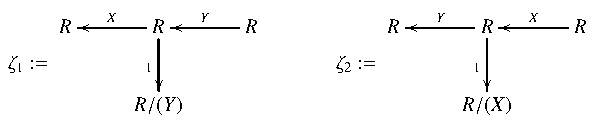
\includegraphics[width=0.78\textwidth]{figures/Fig_216_PDF319_Book307.pdf}
  \caption{两条次数为 $1$ 的 Ext 态射（原书 p.307）}\label{fig:two-lines-degree-one-morphisms}
\end{figure}
\[
  0\longrightarrow R/(X)\xrightarrow{\,Y\,}R\xrightarrow{\,X\,}R/(Y)\longrightarrow0,
  \qquad
  0\longrightarrow R/(Y)\xrightarrow{\,X\,}R\xrightarrow{\,Y\,}R/(X)\longrightarrow0.
\]
所得 Ext 代数作为 $A_\infty$ 代数同构于裤子曲面对应的标准温和代数。三个模生成 $D\mathrm{Mod}^{\bullet}(\mathbb C[X,Y]/(XY))$，故两侧范畴等价。
\hfill$\square$
\end{proof}
% [Tutor Note: 原书 p.307 把两个短正合列都印成 $0\to R/(X)\xrightarrow{Y}R\xrightarrow{X}R/(Y)\to0$；由 $\zeta_2$ 的图，第二个应为 $0\to R/(Y)\xrightarrow{X}R\xrightarrow{Y}R/(X)\to0$。译文已改正，否则无法同时得到 $R/(X)$ 与 $R/(Y)$ 的两种锥，Ext 代数也少两个生成元。]

可以把这个分次曲面想成 $\mathbb C\setminus\{0,1\}$，其线场沿径向向外。图\ref{fig:two-lines-mirror-picture} 中，$R$ 对应实区间 $(-\infty,0)$，$R/(X)$ 对应 $(0,1)$，而 $R/(Y)$ 对应 $(1,+\infty)$。
\begin{figure}[H]\centering
  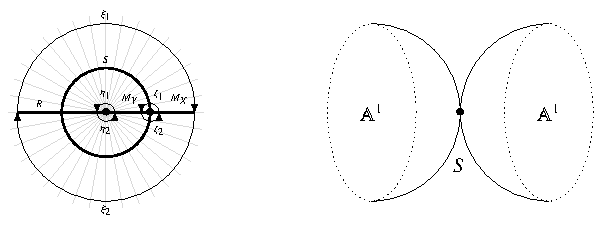
\includegraphics[width=0.9\textwidth]{figures/Fig_217_PDF319_Book307.pdf}
  \caption{裤子曲面与相交仿射直线的镜像对应（原书 p.307）}\label{fig:two-lines-mirror-picture}
\end{figure}

位于第一条仿射直线 $\mathbb A^1=V(R/(X))$ 上的点，其点层
\[
  R/(X,Y-\lambda)
\]
对应于单位圆盘内圆周上的带对象。第二条仿射直线 $\mathbb A^1=V(R/(Y))$ 上的点层 $R/(Y,X-\lambda)$ 也对应于单位圆盘内圆周上的带对象。奇点
\[
  S=R/(X,Y)
\]
处的点层则对应于单位圆上的弦对象。

\begin{example}[直线链]\label{ex:chain-of-lines}
考虑带相同线场的 $(\mathbb P^1,\{0,\infty,1,\ldots,k\})$。沿着相邻的 $k$ 个标记点之间的圆周切开曲面，可将它看成 $k$ 枚裤子曲面沿带对象粘合。$B$ 侧则把两条相交于原点的仿射直线沿开子集 $\mathbb C^*$ 粘合。两条仿射直线粘合后成为一条射影直线，因此得到一条由仿射直线和射影直线组成的链：
\[
  \mathbb A^1_0\sqcup_\infty\mathbb P^1_0\sqcup_\infty\cdots
  \sqcup_\infty\mathbb P^1_0\sqcup_0\mathbb A^1.
\]
\begin{figure}[H]\centering
  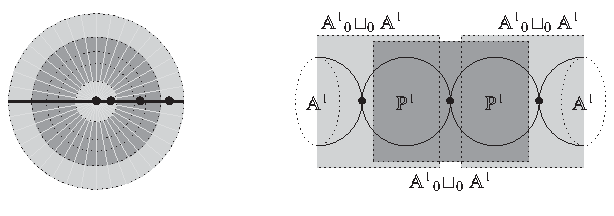
\includegraphics[width=0.95\textwidth]{figures/Fig_218_PDF319_Book307.pdf}
  \caption{裤子曲面粘合与直线链（原书 p.307）}\label{fig:chain-of-lines-gluing}
\end{figure}

还可以用另一种方式粘合：沿穿过标记点的圆周切开曲面，将它分成若干圆柱，再沿弦对象粘合这些圆柱。两端的部分是一个圆盘，其中有一个内部标记点和一个边界标记点，对应 $B$ 侧的一条仿射直线；中间部分是两侧边界各有一个标记点的圆柱，对应 $A$ 侧的一条射影直线。由于沿弦对象粘合，在 $B$ 侧只需把相应点识别起来，所得仍是同一条链（见图\ref{fig:chain-of-lines-second-gluing}）。省去一端或两端包含 $0$、$\infty$ 的部分，还可得到只有一个仿射分支或完全没有仿射分支的链。
\begin{figure}[H]\centering
  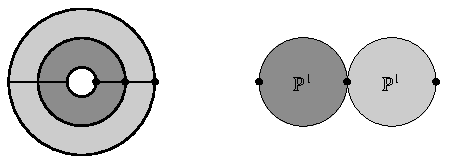
\includegraphics[width=0.60\textwidth]{figures/Fig_219_PDF320_Book308.pdf}
  \caption{沿弦对象粘合的圆柱与射影直线链（原书 p.308）}\label{fig:chain-of-lines-second-gluing}
\end{figure}
\end{example}

\begin{example}[射影直线的环链]
现在考虑环面 $\mathbb C/(\mathbb Z+i\mathbb Z)$，其内部有 $k>1$ 个标记点，并取水平线场。仍可沿切割把环面分成含内部标记点的圆柱，或分成两侧各有一个标记点的圆柱。两种切法都得到由 $k$ 条射影直线构成的环链，如图\ref{fig:necklace-of-lines}。
\begin{figure}[H]\centering
  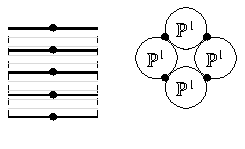
\includegraphics[width=0.37\textwidth]{figures/Fig_220_PDF320_Book308.pdf}
  \caption{环面上的射影直线环链（原书 p.308）}\label{fig:necklace-of-lines}
\end{figure}
\end{example}

\begin{example}[结点三次曲线]
考虑仅有一个内部标记点、带水平线场的环面 $\mathbb C/(\mathbb Z+i\mathbb Z)$。此时必须把一条射影直线上的两个点粘合起来，所得是结点曲线 $E$。它可表示为射影平面 $\mathbb P^2$ 中方程
\[
  Y^2Z-XYZ-X^3=0
\]
的零点集。$E$ 上有两个生成范畴的对象：奇点 $s=(0:0:1)$ 处的点层 $S$，与结构层 $\mathcal O$。在 $A$ 侧，这两个对象分别对应于从标记点出发又回到该点的竖直弦对象，和水平带对象。该例见文献\bookcite{162}。
\begin{figure}[H]\centering
  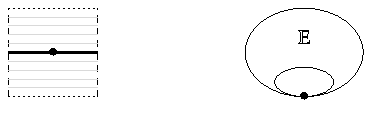
\includegraphics[width=0.55\textwidth]{figures/Fig_221_PDF321_Book309.pdf}
  \caption{结点三次曲线及其两个生成对象（原书 p.309）}\label{fig:nodal-cubic-generators}
\end{figure}
\end{example}

\section{镜像轨形簇}\label{sec:mirror-orbifolds}
\takeaway{奇点轨形 $[\mathbb A^1_0\sqcup_0\mathbb A^1/\mathbb Z_k]_r$ 的导出范畴是 $\mathbb C[X,Y]/(XY)\star\mathbb Z_k$ 的模范畴，其箭图有 $k$ 个顶点与两条出箭 $X_i,Y_i$；$A$ 侧是两个圆盘沿边界弧粘合所得曲面，亏格 $(k-m)/2$ 由移位 $u\mapsto u+1+r$ 的轨道数 $m$ 决定。}
如果 $B$ 侧只允许簇，则无法为亏格 $g\ge2$ 的曲面找到镜像。使用轨形或栈可以绕过这一限制，也为亏格 $g\ge2$ 的情形构造新的镜像。

在 $B$ 侧，考虑奇点轨形
\[
  [\mathbb A^1_0\sqcup_0\mathbb A^1/\mathbb Z_k]_r,
\]
其中 $\mathbb Z_k$ 在第一条直线上按乘以 $e^{2\pi i/k}$ 的方式作用，在第二条直线上按乘以 $e^{2r\pi i/k}$ 的方式作用，且 $r\in\mathbb Z_k^*$。按定义，该栈的导出范畴是代数
\[
  A=\mathbb C[X,Y]/(XY)\star\mathbb Z_k
\]
的模导出范畴。这个代数同构于一个带关系的箭图的路径代数：箭图由一个有 $k$ 个顶点 $v_i$ 的环组成，每个顶点有两条出箭
\[
  X_i\colon v_i\to v_{i+1},\qquad
  Y_i\colon v_i\to v_{i+r},
\]
其中下标按模 $k$ 计算；关系为
\[
  Y_{i+1}X_i=0,\qquad X_{i+r}Y_i=0.
\]

构造 $A$ 模型时，取两个圆盘，每个圆盘内部各有一个标记点，边界上各有 $k$ 个标记点，并在其上取径向线场。在第一个圆盘上，按逆时针方向将边界弧记为 $c_i$（$i\in\{1,\ldots,k\}$）；第二个圆盘上的弧记为 $c_{ri}$，下标按模 $k$ 计算。将名称相同的弧粘合，所得是一个无边界的定向曲面，其内部标记点数为 $2+m$：前两个是原来两个圆盘的中心，而 $m$ 是 $\mathbb Z_k$ 在变换
\[
  u\longmapsto u+1+r
\]
下的轨道数。这个轨道数也等于由 $X,Y$ 箭交替组成的箭图环路数（锯齿路径数）。所得曲面由两个 $k$ 边形和 $m$ 个角组成，亏格为
\[
  g=\frac{k-m}{2}.
\]
由于沿多边形内部角传递线场时变化量为 $\pi$，绕任一内部标记点转一整周的总次数为 $2k/m$。
% [Tutor Note: 这里的轨道数 $m$ 同时是内部标记点数与锯齿路径数：移位 $u\mapsto u+1+r$ 在 $\mathbb Z_k$ 上的轨道数决定亏格 $g=(k-m)/2$，所以改变 $r$ 就得到不同亏格的镜像曲面；例 10.11 中 $r=3,4$（$k=5$）分别给出 $m=1$ 与 $m=5$，即 $g=2$ 与 $g=0$。]

在多边形的边上再添连接圆盘中心与边界标记点的径向弧，即得到弧系 $A$。在镜像对应下，多边形边对应于简单顶点表示 $v_iA/(X,Y)$，径向弧对应于模 $v_iA/(X)$ 和 $v_iA/(Y)$。这 $3k$ 个模生成 $D\mathrm{Mod}^{\bullet}A$，它们直和的 Ext 环作为 $A_\infty$ 代数同构于温和代数 $\mathrm{Gtl}^{\bullet}A$。改变 $r$ 即可得到不同曲面。

\begin{example}[五阶循环群作用]\label{ex:cyclic-k5}
取 $k=5$，分别令 $r=3,4$。第一种情形的亏格为 $2$，第二种情形的亏格为 $0$，见图\ref{fig:orbifold-mirrors-k5}。
\begin{figure}[H]\centering
  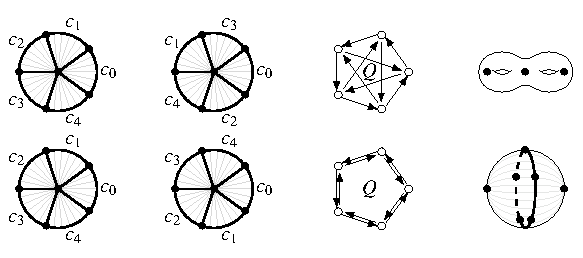
\includegraphics[width=0.85\textwidth]{figures/Fig_222_PDF322_Book310.pdf}
  \caption{$k=5,r=3$ 与 $r=4$ 时的镜像曲面（原书 p.310）}\label{fig:orbifold-mirrors-k5}
\end{figure}

一般地，若 $r=k-1$，则亏格恒为 $0$，所得曲面是
\[
  \mathbb C^*\setminus\{e^{2j\pi i/k}\mid j\in\mathbb Z\}
\]
的镜像。这个分次曲面等价于 $\mathbb C^*\setminus\{1,\ldots,k\}$，所以轨形奇点的导出范畴等价于由两条仿射直线和 $k-1$ 条射影直线组成的链的相干层导出范畴。于是得到两个 $B$ 模型之间的非平凡对应：
\[
  D\mathrm{Coh}^{\bullet}[\mathbb A^1_0\sqcup_0\mathbb A^1/\mathbb Z_k]_{k-1}
\cong_\infty
  D\mathrm{Coh}^{\bullet}\bigl(\mathbb A^1_0\sqcup_0\mathbb P^1_\infty
  \sqcup_0\cdots\sqcup_0\mathbb P^1_\infty\sqcup_0\mathbb A^1\bigr).
\]
还可以将这类轨形粘合成链或环，从而构造更多类似的镜像等价。Lekili 和 Polishchuk 在文献\bookcite{165}中详细研究了这些构造。
\end{example}

\section{习题}\label{sec:grading-exercises}

\begin{exercise}\label{exer:grading-closed-surface-existence}
证明：没有标记点的闭曲面 $S$ 只有在亏格为 $1$ 时才存在全局线场。
\end{exercise}

\begin{exercise}\label{exer:grading-index-theorem-wedges}
设 $S$ 是带标记点 $M$ 的闭曲面，$S\setminus M$ 上有线场 $V$。假设存在一组叶构成的弧系，并且它将曲面剖分。证明：若用楔形区域计数公式计算标记点指标，则 Poincaré 指标定理成立。
\end{exercise}

\begin{exercise}\label{exer:grading-contractible-loop}
设 $S$ 是带标记点 $M$ 的闭曲面，$\gamma$ 是 $S$ 中一条可缩闭曲线，并围成圆盘 $U$。$U$ 内标记点的指标须满足什么条件，$\gamma$ 才可分次？
\end{exercise}

\begin{exercise}\label{exer:grading-linear-gentle-algebra}
找一个分次曲面及其弧系，使相应温和代数是下图箭图的分次路径代数：
\begin{figure}[H]\centering
  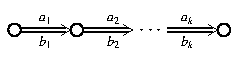
\includegraphics[width=0.35\textwidth]{figures/Fig_223_PDF322_Book310.pdf}
  \caption{习题 10.4 中的箭图（原书 p.310）}\label{fig:grading-linear-exercise-quiver}
\end{figure}
关系为
\[
  a_{i+1}a_i=b_{i+1}b_i=0,
\]
且 $\deg a_i=1$、$\deg b_i=0$。
\end{exercise}

\begin{exercise}\label{exer:grading-three-arrow-quiver}
考虑下图所示、无关系的箭图：
\begin{figure}[H]\centering
  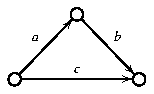
\includegraphics[width=0.24\textwidth]{figures/Fig_224_PDF323_Book311.pdf}
  \caption{习题 10.5 中的箭图（原书 p.311）}\label{fig:grading-three-arrow-quiver}
\end{figure}
对每个次数三元组
\[
  (\deg a,\deg b,\deg c)\in\mathbb Z^3,
\]
求一个分次曲面及其弧系 $A$，使温和代数成为该箭图的分次路径代数。描述 $D\mathrm{Gtl}^{\bullet}A$ 中不可分解对象，并区分不同的次数三元组。
\end{exercise}

\begin{exercise}\label{exer:grading-nonzero-arf-genus-two}
构造一个亏格为 $2$ 且 Arf 不变量非零的分次曲面。
\end{exercise}

\begin{exercise}\label{exer:grading-reflexive-polygon-torus}
设 $\square$ 是带三角剖分 $\boxtimes$ 的反射多边形，$v_0$ 是其中的内部格点。元素 $2v_0\in N=\mathbb Z^3$ 在 $\mathbb C[M]$ 上定义分次 $\deg_{2v_0}$，并且
\[
  \deg_{2v_0}\ell=2.
\]
因此，可以用它为 $(X_{\boxtimes}^{3},\ell)$ 的矩阵分解范畴定义分次。证明：相应的分次带标记曲面是带二次微分 $(dz)^2$ 的环面。
\end{exercise}

\begin{exercise}\label{exer:grading-perfect-matching-line-field}
设 $Q$ 是环面上的一致二聚体模型。完美匹配 $P\subset Q_1$ 是一组箭，并且每个 $Q_2$ 中的环路恰好包含 $P$ 中的一条箭。利用它定义 $\mathrm{Jac}(Q)$ 上的分次 $\deg_{2P}$：对属于 $P$ 的箭赋予次数 $2$，其他箭赋予次数 $0$。此分次满足 $\deg_{2P}\ell=2$，因而可用于为 $(\mathrm{Jac}(Q),\ell)$ 的矩阵分解范畴定义分次。构造 $Q^\vee$ 上与该分次互为镜像的线场。
\end{exercise}

\begin{exercise}\label{exer:grading-orbifold-necklace}
设 $X$ 是由 $k$ 条 $\mathbb P^1$ 构成的环链。构造与 $X$ 导出等价的轨形栈。这样的构造有多少种？
\end{exercise}

\begin{exercise}\label{exer:grading-cylinder-orbifold-points}
设 $S$ 是一个圆柱，一侧边界上有 $k$ 个标记点，另一侧也有 $k$ 个标记点。给 $S$ 配备平行于圆柱轴线的线场。它在 $B$ 侧的镜像应是带两个轨形点的射影直线。将其导出范畴构造成某个代数层的模层导出范畴。
\end{exercise}

\chapterreview{%
\textbf{全章地位。}第 9 章用弧系的路径代数造出 $\mathbb Z_2$ 分次的拓扑 Fukaya 范畴，本章把它提升到 $\mathbb Z$ 分次。这一步不只是加细：有了整数分次，矩阵分解才能换成分次矩阵分解，$B$ 侧才能给出真正的（可能奇异的）簇，而不只是 Landau--Ginzburg 模型。本章取材于 Haiden--Katzarkov--Kontsevich 与 Lekili--Polishchuk，技术密度为全书之最。

\textbf{知识脉络。}线索是“几何 $\to$ 拓扑 $\to$ 代数 $\to$ 镜像”。§10.1 用线场（射影切丛 $PT\dot S$ 的截面）定义相位提升，把分次问题化为绕数 $w$ 是否为零；$I_m=1-w/2$ 与 Poincaré 指标定理给出整体约束，角态射的分次与 $\mu^k$ 的次数 $2-k$ 也在此给出。§10.2 由此得到弦对象、带对象的分次规则与分解定理。§10.3 给出分类：两个分次曲面何时等价，由奇偶性、绕数向量 $W$、$g=1$ 的 $\mathrm{GCD}$ 与 $g\ge2$ 的 $\mathrm{ARF}$ 决定。§10.4 转向 $B$ 侧，以 $\deg Z=2-\deg X-\deg Y$ 固定势函数的次数为 $2$，得到分次裤子曲面的镜像。§10.5、§10.6 放宽奇点条件，得到直线链、射影直线环链、结点三次曲线与轨形 $[\mathbb A^1_0\sqcup_0\mathbb A^1/\mathbb Z_k]_r$ 的镜像。

\textbf{核心结论。}（1）$\vec L[n]=(L,\theta+n\pi)$，平移加的是半圈；闭曲线可分次当且仅当 $w(\eta,L)=0$，而 $\sum_m(1-w(\eta,\gamma_m)/2)=2-2g$ 是 Poincaré 指标定理的分次版本。（2）角态射分次为 $\deg_{\vec A}\alpha=(\Delta_\alpha-(\theta_b(p)-\theta_a(p)))/\pi$，$\mu^k$ 的次数为 $2-k$；弦对象的平移须满足 $i_{j+1}=i_j+\deg\alpha_j-1$，带对象存在当且仅当 $\sum_j(\deg\alpha_j-1)=0$，且 $D\mathrm{Gtl}^{\bullet}\vec A$ 中每个对象都同构于弦与带的直和。（3）$(\mathbb P^1,\{0,\infty,1\},z^k(z-1)^l dz^2)$ 的镜像是 $(\mathbb C[X,Y,Z],XYZ)$，$\deg X=2+k$、$\deg Y=-k-l-2$、$\deg Z=2+l$；更一般地 $\deg X=2-2I_{m_\xi}$ 把 $A$ 侧指标翻译成 $B$ 侧变量次数。（4）当各标记点绕数只取 $0$ 或 $2$ 时，$\mathrm{topFuk}^{\bullet}$ 等价于真簇的导出范畴：裤子对应 $D\mathrm{Coh}^{\bullet}(\mathbb A^1\cup_p\mathbb A^1)\cong D\mathrm{Mod}^{\bullet}\mathbb C[X,Y]/(XY)$；轨形对应 $\mathbb C[X,Y]/(XY)\star\mathbb Z_k$ 的模范畴，亏格为 $(k-m)/2$。

\textbf{辨析与提醒。}其一，线场无向，相位只在模 $\pi$ 意义下有定义，所以平移加 $n\pi$；这正是 $\mathbb Z$ 分次比 $\mathbb Z_2$ 分次多出的“半圈信息”。其二，指标与绕数的换算 $I_m=1-w/2$ 要记牢：$w=0$ 对应 $I=1$，$w=2$ 对应 $I=0$；Poincaré 约束意味着 $g=0$ 时恰有两个 $w=0$ 的点，$g=1$ 时可以没有，这决定了 §10.5 中哪些曲面能给出真簇。其三，弦对象的分次是递推的，不能给每个直和项任意加平移；带对象要求总次数恰为零，否则整体相位不存在。其四，$A$ 侧的分次是拓扑数据，$B$ 侧的分次是代数数据，两者通过 $\deg Z=2-\deg X-\deg Y$（即 $\mu^0$ 次数为 $2$）对接；改变轨形参数 $r$ 会改变轨道数 $m$，从而得到不同亏格，例~\ref{ex:cyclic-k5} 中 $k=5$、$r=3,4$ 分别给出亏格 $2$ 与 $0$。

\textbf{评注。}本章的骨架是 HKK 的分解定理：每个对象都是弦与带的直和。它把 $\mathbb Z_2$ 情形下“对象即弧系”的直觉推广到分次情形，使计算归结为曲线上的局部系统与绕数。Lekili--Polishchuk 的分类则给出少见的“完全分类”：两个分次曲面是否等价，只看奇偶性、绕数向量与 $\mathrm{GCD}$、$\mathrm{ARF}$ 这几个整数；作者把它放在 §10.3 而非末尾，是为了让读者进入 $B$ 侧前就掌握判据。本章只处理拓扑二维的带标记曲面，不涉及高维辛几何中的分次与 $Spin$ 结构，这一限制使证明初等、结论干净。阅读时建议手算两例：三标记球面检验分次与 $\mathbb Z_2$ 分次是否相容，四穿孔球面检验粘合时整周角次数互为相反数的条件；这两例算通，§10.5 的直线链与环链就只是机械推广。}
